\section{Numeri complessi}

% TODO: aggiungere grafici dove vi è un TODO vuoto

\subsection{Costruzione}

\begin{definition}[Campo complesso]
  $$\complex\walrus\reals\times\reals=\reals^2$$
  $$\complex\ni z\walrus\(a,b\)\in\reals^2$$
  \begin{center}
    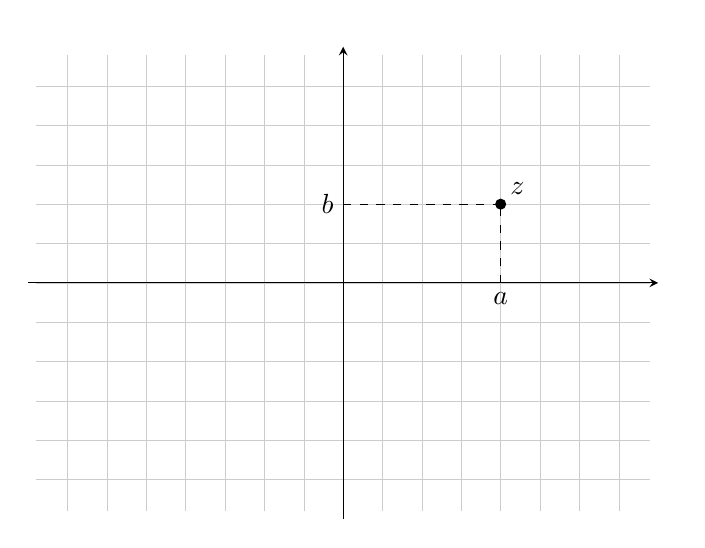
\begin{tikzpicture}
      \def\a{2};
      \def\b{1};
      \draw [black!20,step=0.5,very thin] (-4+0.1,-3+0.1) grid (4-0.1,3-0.1);
      \draw[-stealth] (-4,0) -- (4,0) node [right] {$\reals$};
      \draw[-stealth] (0,-3) -- (0,3) node [above] {$\reals$};
      \fill (\a,\b) circle (2pt);
      \draw (\a,\b) node [above right] {$z$};
      \draw[dashed] (0,\b) -- (\a,\b);
      \draw[dashed] (\a,0) -- (\a,\b);
      \draw (\a,0) node [below] {$a$};
      \draw (0,\b) node [left] {$b$};
      \draw (-2,-1.5) node {$\complex$};
    \end{tikzpicture}
  \end{center}
\end{definition}

\begin{definition}[Somma in $\complex$]
  $$z,w\in\complex$$
  $$z\walrus\(a,b\)$$
  $$w\walrus\(c,d\)$$
  $$z+w\walrus\(a+c,b+d\)$$
  \begin{center}
    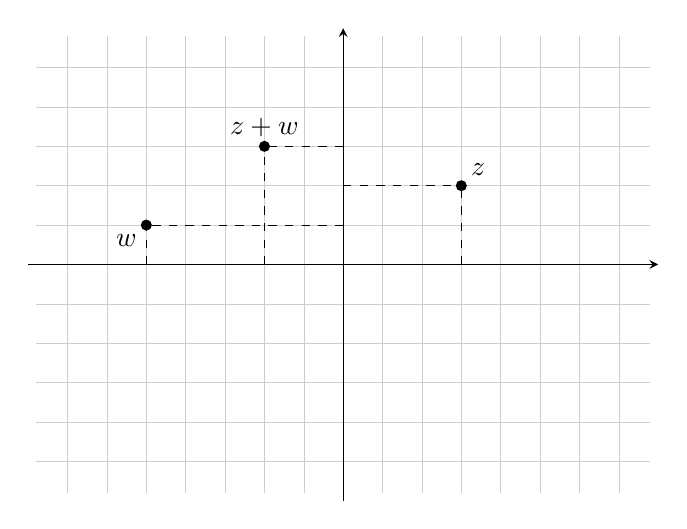
\begin{tikzpicture}
      \def\a{1.5};
      \def\b{1};
      \def\c{-2.5};
      \def\d{0.5};
      \draw [black!20,step=0.5,very thin] (-4+0.1,-3+0.1) grid (4-0.1,3-0.1);
      \draw[-stealth] (-4,0) -- (4,0);
      \draw[-stealth] (0,-3) -- (0,3);
      \fill (\a,\b) circle (2pt);
      \draw (\a,\b) node [above right] {$z$};
      \draw[dashed] (0,\b) -- (\a,\b);
      \draw[dashed] (\a,0) -- (\a,\b);
      % \draw (\a,0) node [below] {$a$};
      % \draw (0,\b) node [left] {$b$};
      \fill (\c,\d) circle (2pt);
      \draw (\c,\d) node [below left] {$w$};
      \draw[dashed] (0,\d) -- (\c,\d);
      \draw[dashed] (\c,0) -- (\c,\d);
      % \draw (\c,0) node [above] {$c$};
      % \draw (0,\d) node [right] {$d$};
      \fill (\a+\c,\b+\d) circle (2pt);
      \draw (\a+\c,\b+\d) node [above] {$z+w$};
      \draw[dashed] (0,\b+\d) -- (\a+\c,\b+\d);
      \draw[dashed] (\a+\c,0) -- (\a+\c,\b+\d);
      % \draw (\a+\c,0) node [below] {$a+c$};
      % \draw (0,\b+\d) node [right] {$b+d$};
    \end{tikzpicture}
  \end{center}
\end{definition}

\begin{definition}[Prodotto in $\complex$]
  $$z,w\in\complex$$
  $$z\walrus\(a,b\)$$
  $$w\walrus\(c,d\)$$
  $$z\cdot w\walrus\(ac-bd,ad+bc\)$$
  \begin{center}
    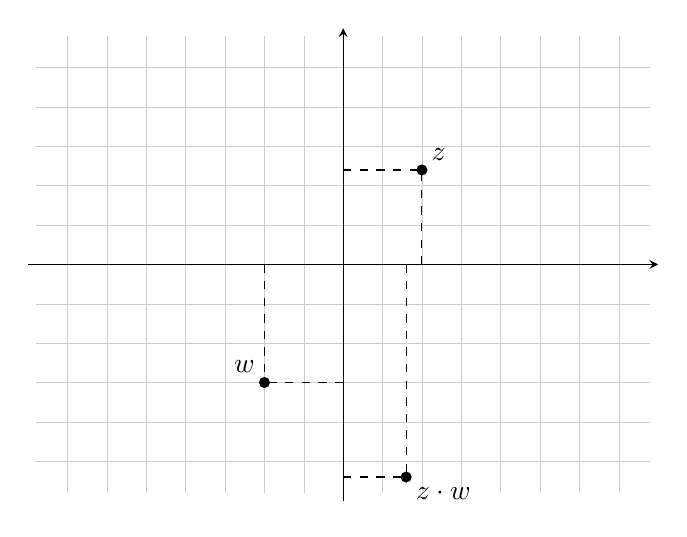
\begin{tikzpicture}
      \def\a{1};
      \def\b{1.2};
      \def\c{-1};
      \def\d{-1.5};
      \draw [black!20,step=0.5,very thin] (-4+0.1,-3+0.1) grid (4-0.1,3-0.1);
      \draw[-stealth] (-4,0) -- (4,0);
      \draw[-stealth] (0,-3) -- (0,3);
      \fill (\a,\b) circle (2pt);
      \draw (\a,\b) node [above right] {$z$};
      \draw[dashed] (0,\b) -- (\a,\b);
      \draw[dashed] (\a,0) -- (\a,\b);
      % \draw (\a,0) node [below] {$a$};
      % \draw (0,\b) node [left] {$b$};
      \fill (\c,\d) circle (2pt);
      \draw (\c,\d) node [above left] {$w$};
      \draw[dashed] (0,\d) -- (\c,\d);
      \draw[dashed] (\c,0) -- (\c,\d);
      % \draw (\c,0) node [above] {$c$};
      % \draw (0,\d) node [right] {$d$};
      \fill (\a*\c-\b*\d,\a*\d+\b*\c) circle (2pt);
      \draw (\a*\c-\b*\d,\a*\d+\b*\c) node [below right] {$z\cdot w$};
      \draw[dashed] (0,\a*\d+\b*\c) -- (\a*\c-\b*\d,\a*\d+\b*\c);
      \draw[dashed] (\a*\c-\b*\d,0) -- (\a*\c-\b*\d,\a*\d+\b*\c);
      % \draw (\a*\c-\b*\d,0) node [below] {$ac-bd$};
      % \draw (0,\a*\d+\b*\c) node [right] {$ad+bc$};
    \end{tikzpicture}
  \end{center}
\end{definition}

\subsubsection*{Proprietà}

\begin{itemize}
  \item $z+w=w+z$
  \item $zw=wz$
  \item $z+\(w+v\)=\(z+w\)+v$
  \item $z\(wv\)=\(zw\)v$
  \item $z\(w+t\)=zw+zt$
\end{itemize}

\begin{observation}
  L'elemento neutro della somma è $\(0,0\)$, mentre quello del prodotto è $\(1,0\)$.
\end{observation}
\begin{proof}
  $$\complex\ni z\walrus\left( a,b \right)$$
  $$z+\left( 0,0 \right)=\left( a+0,b+0 \right)=\left( a,b \right)=z$$
  $$z\cdot\left( 1,0 \right)=\left( a\cdot1-b\cdot0,a\cdot0+b\cdot1 \right)=\left( a,b \right)=z$$
\end{proof}

\paragraph*{Immersione di $\reals$ in $\complex$}
$$f:\reals\to\complex\quad f\(x\)\walrus\(x,0\)$$
Sia $f$ iniettiva:
$$f(x)=f(y)\iff \(x,0\)=\(y,0\)\iff x=y$$
Allora:
$$f(x)+f(y)=\(x,0\)+\(y,0\)=\(x+y,0\)=f(x+y)$$
$$f(x)f(y)=\(x,0\)\(y,0\)=\(xy-0,0+0\)=f(xy)$$

\subsection{Forma algebrica}

$$z=\(a,b\)\in\complex$$
$$\complex \ni i\walrus\(0,1\)$$
\begin{align*}
  z & =\(a,b\)             \\
    & =\(a,0\)+\(0,b\)     \\
    & =f(a)+\(0,1\)\(b,0\) \\
    & =f(a)+\(0,1\)f(b)    \\
    & =a+\(0,1\)b          \\
    & =a+ib                
\end{align*}

\begin{observation}
  $$i^2=\(0,1\)\(0,1\)=\(0-1,0+0\)=f(-1)=-1\iff i^2+1=0$$
\end{observation}

\subsection{Operazioni}

$$\(a+ib\)+\(c+id\)=\(a+c\)+i\(b+d\)$$
$$\(a+ib\)+\(c+id\)=\(ac-bd\)+i\(ad+bc\)$$
\begin{definition}[Negazione in $\complex$]
  $$-\(a+ib\)\walrus-a-ib$$
  \begin{center}
    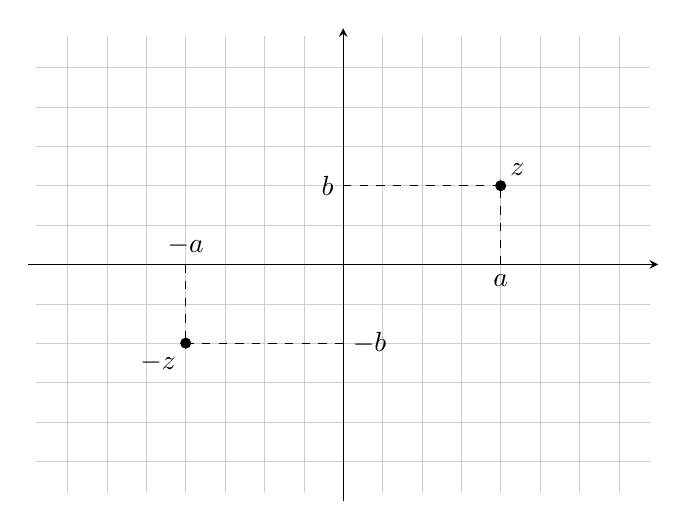
\begin{tikzpicture}
      \def\a{2};
      \def\b{1};
      \draw [black!20,step=0.5,very thin] (-4+0.1,-3+0.1) grid (4-0.1,3-0.1);
      \draw[-stealth] (-4,0) -- (4,0);
      \draw[-stealth] (0,-3) -- (0,3);
      \fill (\a,\b) circle (2pt);
      \draw (\a,\b) node [above right] {$z$};
      \draw[dashed] (0,\b) -- (\a,\b);
      \draw[dashed] (\a,0) -- (\a,\b);
      \draw (\a,0) node [below] {$a$};
      \draw (0,\b) node [left] {$b$};
      \fill (-\a,-\b) circle (2pt);
      \draw (-\a,-\b) node [below left] {$-z$};
      \draw[dashed] (0,-\b) -- (-\a,-\b);
      \draw[dashed] (-\a,0) -- (-\a,-\b);
      \draw (-\a,0) node [above] {$-a$};
      \draw (0,-\b) node [right] {$-b$};
    \end{tikzpicture}
  \end{center}
\end{definition}

\begin{definition}[Reciproco in $\complex$]
  $$z^{-1}\walrus\frac{1}{z}=\frac{1}{a+ib}=\frac{a}{a^2+b^2}-i\frac{b}{a^2+b^2}$$
  \begin{center}
    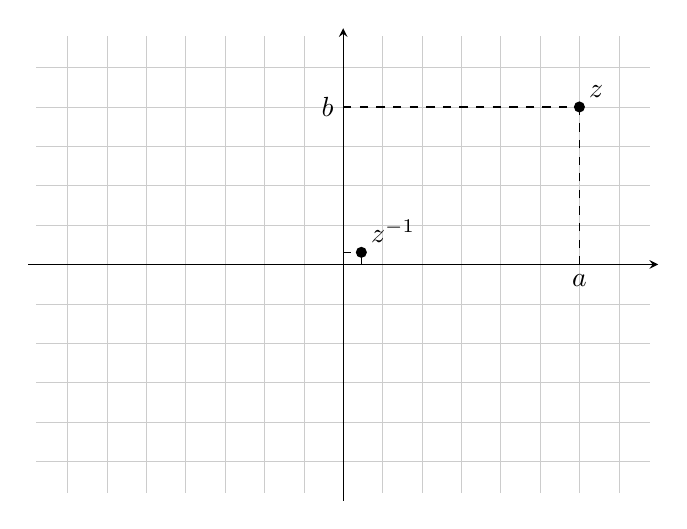
\begin{tikzpicture}
      \def\a{3};
      \def\b{2};
      \draw [black!20,step=0.5,very thin] (-4+0.1,-3+0.1) grid (4-0.1,3-0.1);
      \draw[-stealth] (-4,0) -- (4,0);
      \draw[-stealth] (0,-3) -- (0,3);
      \fill (\a,\b) circle (2pt);
      \draw (\a,\b) node [above right] {$z$};
      \draw[dashed] (0,\b) -- (\a,\b);
      \draw[dashed] (\a,0) -- (\a,\b);
      \draw (\a,0) node [below] {$a$};
      \draw (0,\b) node [left] {$b$};
      \fill ({\a/(\a^2+\b^2)},{\b/(\a^2+\b^2)}) circle (2pt);
      \draw ({\a/(\a^2+\b^2)},{\b/(\a^2+\b^2)}) node [above right] {$z^{-1}$};
      \draw[dashed] (0,{\b/(\a^2+\b^2)}) -- ({\a/(\a^2+\b^2)},{\b/(\a^2+\b^2)});
      \draw[dashed] ({\a/(\a^2+\b^2)},0) -- ({\a/(\a^2+\b^2)},{\b/(\a^2+\b^2)});
      % \draw ({\a/(\a^2+\b^2)},0) node [above] {$\frac{a}{a^2+b^2}$};
      % \draw (0,{\b/(\a^2+\b^2)}) node [right] {$\frac{b}{a^2+b^2}$};
    \end{tikzpicture}
  \end{center}
\end{definition}

\begin{definition}[Parte reale e immaginaria]
  Sia $\complex\ni z\walrus a+ib$. $a$ è detta \textbf{parte reale} di $z$, mentre $b$ è detta \textbf{parte immaginaria} di $z$. Si indicano rispettivamente con $\re\(z\)$ e $\im\(z\)$.
  \begin{center}
    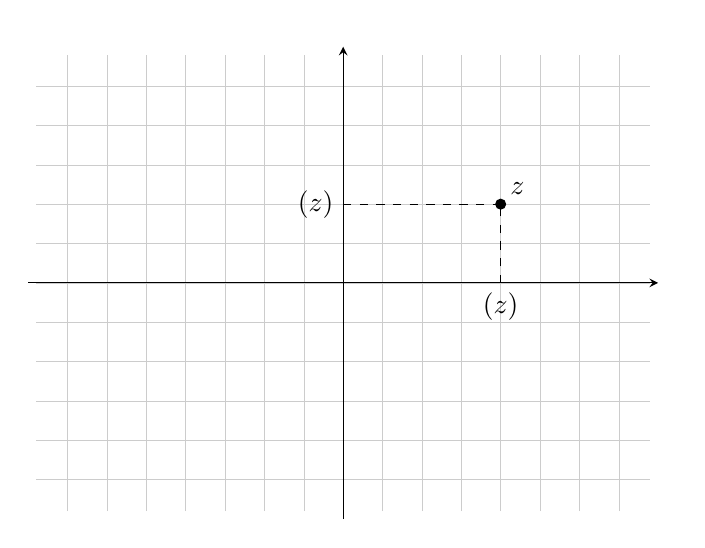
\begin{tikzpicture}
      \def\a{2};
      \def\b{1};
      \draw [black!20,step=0.5,very thin] (-4+0.1,-3+0.1) grid (4-0.1,3-0.1);
      \draw[-stealth] (-4,0) -- (4,0) node [right] {$\re$};
      \draw[-stealth] (0,-3) -- (0,3) node [above] {$\im$};
      \fill (\a,\b) circle (2pt);
      \draw (\a,\b) node [above right] {$z$};
      \draw[dashed] (0,\b) -- (\a,\b);
      \draw[dashed] (\a,0) -- (\a,\b);
      \draw (\a,0) node [below] {$\re\left( z \right)$};
      \draw (0,\b) node [left] {$\im\left( z \right)$};
      \draw (-2,-1.5) node {$\complex$};
    \end{tikzpicture}
  \end{center}
\end{definition}

\begin{definition}[Coniugato]
  Il \textbf{coniugato} di $\complex\ni z\walrus a+ib$ è:
  $$\bar{z}\walrus a-ib$$
  \begin{center}
    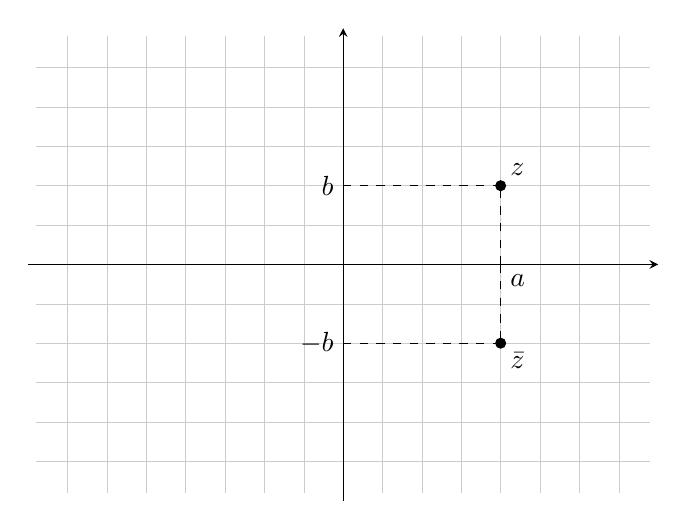
\begin{tikzpicture}
      \def\a{2};
      \def\b{1};
      \draw [black!20,step=0.5,very thin] (-4+0.1,-3+0.1) grid (4-0.1,3-0.1);
      \draw[-stealth] (-4,0) -- (4,0);
      \draw[-stealth] (0,-3) -- (0,3);
      \fill (\a,\b) circle (2pt);
      \draw (\a,\b) node [above right] {$z$};
      \draw[dashed] (0,\b) -- (\a,\b);
      \draw[dashed] (\a,0) -- (\a,\b);
      \draw (\a,0) node [below right] {$a$};
      \draw (0,\b) node [left] {$b$};
      \fill (\a,-\b) circle (2pt);
      \draw (\a,-\b) node [below right] {$\bar{z}$};
      \draw[dashed] (0,-\b) -- (\a,-\b);
      \draw[dashed] (\a,0) -- (\a,-\b);
      \draw (0,-\b) node [left] {$-b$};
    \end{tikzpicture}
  \end{center}
\end{definition}

\begin{definition}[Modulo in $\complex$]
  Sia $\complex\ni z\walrus a+ib$.
  $$\abs{z}=\sqrt{a^2+b^2}$$
  \begin{center}
    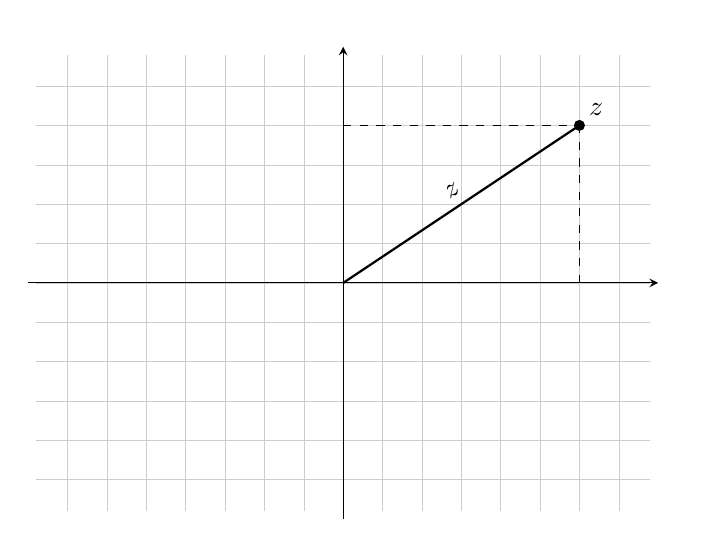
\begin{tikzpicture}
      \def\a{3};
      \def\b{2};
      \draw [black!20,step=0.5,very thin] (-4+0.1,-3+0.1) grid (4-0.1,3-0.1);
      \draw[-stealth] (-4,0) -- (4,0) node [right] {$\re$};
      \draw[-stealth] (0,-3) -- (0,3) node [above] {$\im$};
      \fill (\a,\b) circle (2pt);
      \draw (\a,\b) node [above right] {$z$};
      \draw[dashed] (0,\b) -- (\a,\b);
      \draw[dashed] (\a,0) -- (\a,\b);
      % \draw (\a,0) node [below] {$\re\left( z \right)$};
      % \draw (0,\b) node [left] {$\im\left( z \right)$};
      \draw[thick] (0,0) -- (\a,\b) node [sloped,midway,above] {$\abs{z}$};
    \end{tikzpicture}
  \end{center}
\end{definition}

\begin{observation}
  Mentre $\abs{z}$ è la distanza di $z$ dall'origine, $\abs{z-w}$ è la distanza fra $z$ e $w$.
  \begin{center}
    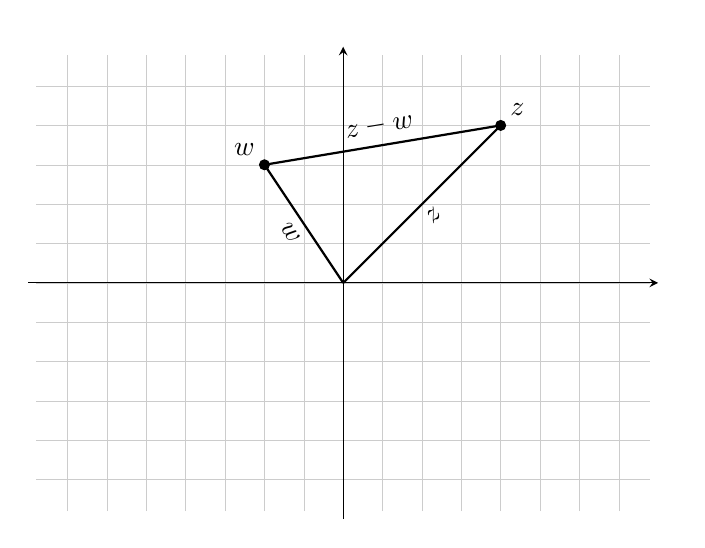
\begin{tikzpicture}
      \def\a{2};
      \def\b{2};
      \def\c{-1};
      \def\d{1.5};
      \draw [black!20,step=0.5,very thin] (-4+0.1,-3+0.1) grid (4-0.1,3-0.1);
      \draw[-stealth] (-4,0) -- (4,0) node [right] {$\re$};
      \draw[-stealth] (0,-3) -- (0,3) node [above] {$\im$};
      \fill (\a,\b) circle (2pt);
      \draw (\a,\b) node [above right] {$z$};
      \draw[thick] (0,0) -- (\a,\b) node [sloped,midway,below] {$\abs{z}$};
      \fill (\c,\d) circle (2pt);
      \draw (\c,\d) node [above left] {$w$};
      \draw[thick] (0,0) -- (\c,\d) node [sloped,midway,below] {$\abs{w}$};
      \draw[thick] (\a,\b) -- (\c,\d) node [sloped,midway,above] {$\abs{z-w}$};
    \end{tikzpicture}
  \end{center}
\end{observation}

\begin{lemma}
  $$\abs{z}=\abs{-z}$$
  \begin{center}
    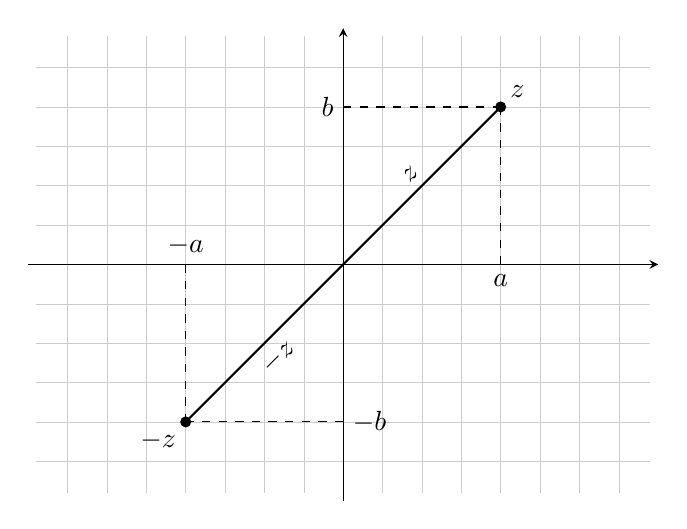
\begin{tikzpicture}
      \def\a{2};
      \def\b{2};
      \draw [black!20,step=0.5,very thin] (-4+0.1,-3+0.1) grid (4-0.1,3-0.1);
      \draw[-stealth] (-4,0) -- (4,0);
      \draw[-stealth] (0,-3) -- (0,3);
      \fill (\a,\b) circle (2pt);
      \draw (\a,\b) node [above right] {$z$};
      \draw[dashed] (0,\b) -- (\a,\b);
      \draw[dashed] (\a,0) -- (\a,\b);
      \draw (\a,0) node [below] {$a$};
      \draw (0,\b) node [left] {$b$};
      \fill (-\a,-\b) circle (2pt);
      \draw (-\a,-\b) node [below left] {$-z$};
      \draw[dashed] (0,-\b) -- (-\a,-\b);
      \draw[dashed] (-\a,0) -- (-\a,-\b);
      \draw (-\a,0) node [above] {$-a$};
      \draw (0,-\b) node [right] {$-b$};
      \draw[thick] (0,0) -- (\a,\b) node [sloped,midway,above] {$\abs{z}$};
      \draw[thick] (0,0) -- (-\a,-\b) node [sloped,midway,below] {$\abs{-z}$};
    \end{tikzpicture}
  \end{center}
\end{lemma}

\begin{lemma}
  $$\abs{z}=\abs{\bar{z}}$$
  \begin{center}
    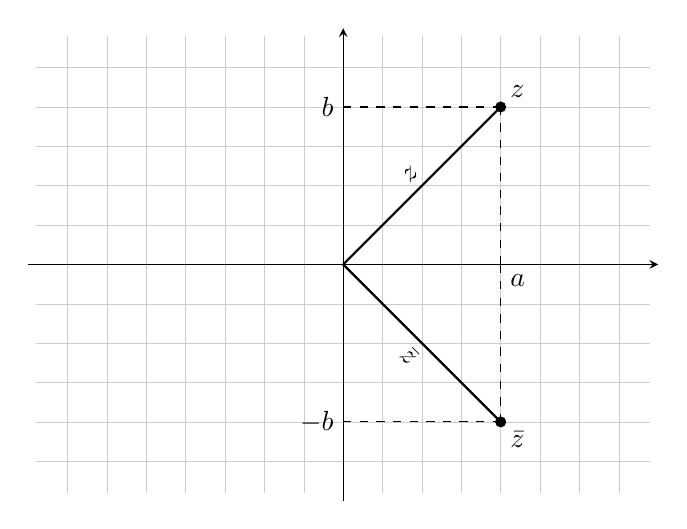
\begin{tikzpicture}
      \def\a{2};
      \def\b{2};
      \draw [black!20,step=0.5,very thin] (-4+0.1,-3+0.1) grid (4-0.1,3-0.1);
      \draw[-stealth] (-4,0) -- (4,0);
      \draw[-stealth] (0,-3) -- (0,3);
      \fill (\a,\b) circle (2pt);
      \draw (\a,\b) node [above right] {$z$};
      \draw[dashed] (0,\b) -- (\a,\b);
      \draw[dashed] (\a,0) -- (\a,\b);
      \draw (\a,0) node [below right] {$a$};
      \draw (0,\b) node [left] {$b$};
      \fill (\a,-\b) circle (2pt);
      \draw (\a,-\b) node [below right] {$\bar{z}$};
      \draw[dashed] (0,-\b) -- (\a,-\b);
      \draw[dashed] (\a,0) -- (\a,-\b);
      \draw (0,-\b) node [left] {$-b$};
      \draw[thick] (0,0) -- (\a,\b) node [sloped,midway,above] {$\abs{z}$};
      \draw[thick] (0,0) -- (\a,-\b) node [sloped,midway,below] {$\abs{\bar{z}}$};
    \end{tikzpicture}
  \end{center}
\end{lemma}

\begin{lemma}
  $$\overline{z+w}=\bar{z}+\bar{w}$$
  \begin{center}
    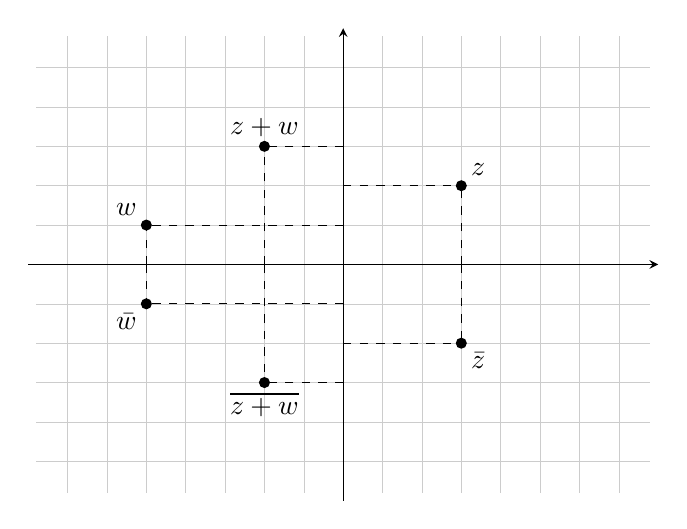
\begin{tikzpicture}
      \def\a{1.5};
      \def\b{1};
      \def\c{-2.5};
      \def\d{0.5};
      \draw [black!20,step=0.5,very thin] (-4+0.1,-3+0.1) grid (4-0.1,3-0.1);
      \draw[-stealth] (-4,0) -- (4,0);
      \draw[-stealth] (0,-3) -- (0,3);
      \fill (\a,\b) circle (2pt);
      \draw (\a,\b) node [above right] {$z$};
      \draw[dashed] (0,\b) -- (\a,\b);
      \draw[dashed] (\a,0) -- (\a,\b);
      \fill (\c,\d) circle (2pt);
      \draw (\c,\d) node [above left] {$w$};
      \draw[dashed] (0,\d) -- (\c,\d);
      \draw[dashed] (\c,0) -- (\c,\d);
      \fill (\a+\c,\b+\d) circle (2pt);
      \draw (\a+\c,\b+\d) node [above] {$z+w$};
      \draw[dashed] (0,\b+\d) -- (\a+\c,\b+\d);
      \draw[dashed] (\a+\c,0) -- (\a+\c,\b+\d);
      \fill (\a,-\b) circle (2pt);
      \draw (\a,-\b) node [below right] {$\bar{z}$};
      \draw[dashed] (0,-\b) -- (\a,-\b);
      \draw[dashed] (\a,0) -- (\a,-\b);
      \fill (\c,-\d) circle (2pt);
      \draw (\c,-\d) node [below left] {$\bar{w}$};
      \draw[dashed] (0,-\d) -- (\c,-\d);
      \draw[dashed] (\c,0) -- (\c,-\d);
      \fill (\a+\c,-\b-\d) circle (2pt);
      \draw (\a+\c,-\b-\d) node [below] {$\overline{z+w}$};
      \draw[dashed] (0,-\b-\d) -- (\a+\c,-\b-\d);
      \draw[dashed] (\a+\c,0) -- (\a+\c,-\b-\d);
    \end{tikzpicture}
  \end{center}
\end{lemma}

\begin{lemma}
  $$\overline{zw}=\bar{z}\bar{w}$$
  \begin{center}
    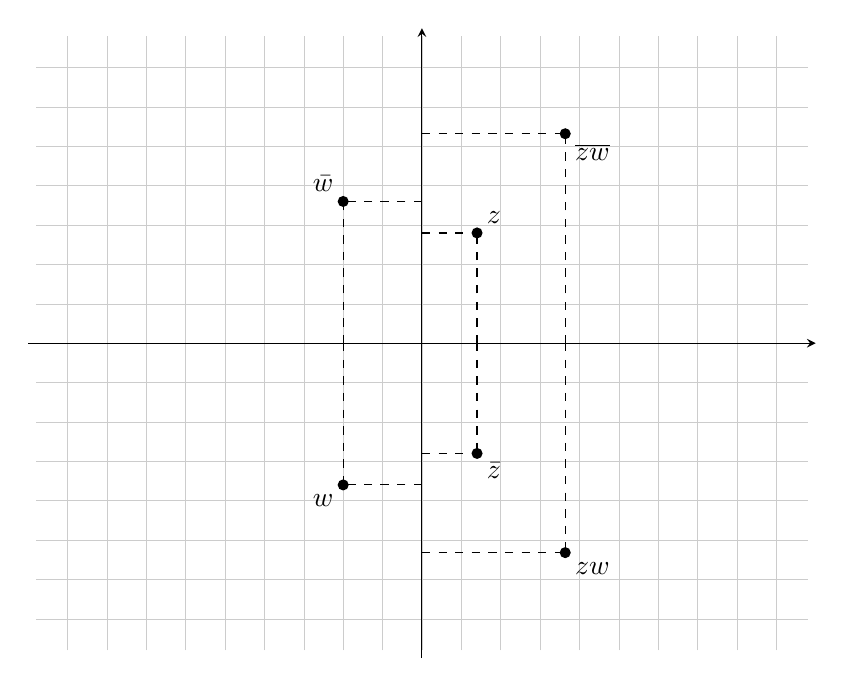
\begin{tikzpicture}
      \def\a{0.7};
      \def\b{1.4};
      \def\c{-1};
      \def\d{-1.8};
      \draw [black!20,step=0.5,very thin] (-5+0.1,-4+0.1) grid (5-0.1,4-0.1);
      \draw[-stealth] (-5,0) -- (5,0);
      \draw[-stealth] (0,-4) -- (0,4);
      \fill (\a,\b) circle (2pt);
      \draw (\a,\b) node [above right] {$z$};
      \draw[dashed] (0,\b) -- (\a,\b);
      \draw[dashed] (\a,0) -- (\a,\b);
      \fill (\c,\d) circle (2pt);
      \draw (\c,\d) node [below left] {$w$};
      \draw[dashed] (0,\d) -- (\c,\d);
      \draw[dashed] (\c,0) -- (\c,\d);
      \fill (\a*\c-\b*\d,\a*\d+\b*\c) circle (2pt);
      \draw (\a*\c-\b*\d,\a*\d+\b*\c) node [below right] {$zw$};
      \draw[dashed] (0,\a*\d+\b*\c) -- (\a*\c-\b*\d,\a*\d+\b*\c);
      \draw[dashed] (\a*\c-\b*\d,0) -- (\a*\c-\b*\d,\a*\d+\b*\c);
      \fill (\a,-\b) circle (2pt);
      \draw (\a,-\b) node [below right] {$\bar{z}$};
      \draw[dashed] (0,-\b) -- (\a,-\b);
      \draw[dashed] (\a,0) -- (\a,-\b);
      \fill (\c,-\d) circle (2pt);
      \draw (\c,-\d) node [above left] {$\bar{w}$};
      \draw[dashed] (0,-\d) -- (\c,-\d);
      \draw[dashed] (\c,0) -- (\c,-\d);
      \fill (\a*\c-\b*\d,{-(\a*\d+\b*\c)}) circle (2pt);
      \draw (\a*\c-\b*\d,{-(\a*\d+\b*\c)}) node [below right] {$\overline{zw}$};
      \draw[dashed] (0,{-(\a*\d+\b*\c)}) -- (\a*\c-\b*\d,{-(\a*\d+\b*\c)});
      \draw[dashed] (\a*\c-\b*\d,0) -- (\a*\c-\b*\d,{-(\a*\d+\b*\c)});
    \end{tikzpicture}
  \end{center}
\end{lemma}

\begin{lemma}
  $$\abs{z}=\sqrt{z\bar{z}}\iff \abs{z}^2=z\bar{z}$$
  \begin{center}
    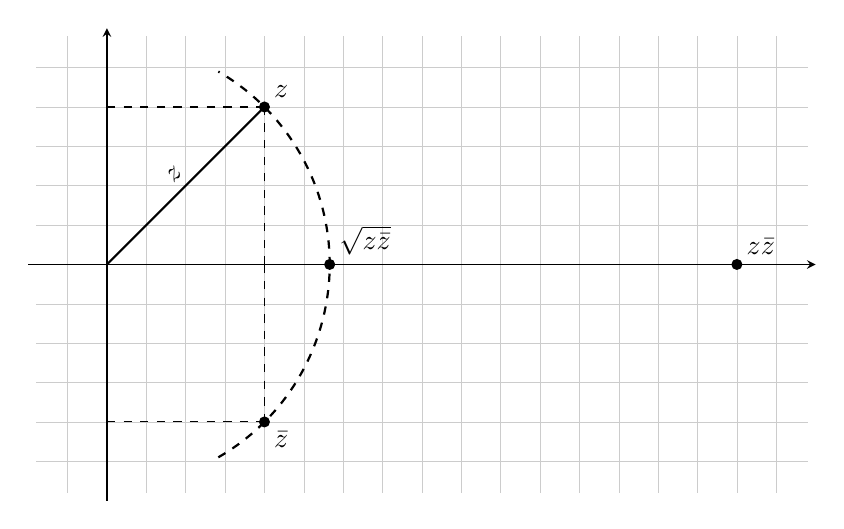
\begin{tikzpicture}
      \def\a{2};
      \def\b{2};
      \draw [black!20,step=0.5,very thin] (-1+0.1,-3+0.1) grid (9-0.1,3-0.1);
      \draw[-stealth] (-1,0) -- (9,0);
      \draw[-stealth] (0,-3) -- (0,3);
      \fill (\a,\b) circle (2pt);
      \draw (\a,\b) node [above right] {$z$};
      \draw[dashed] (0,\b) -- (\a,\b);
      \draw[dashed] (\a,0) -- (\a,\b);
      \fill (\a,-\b) circle (2pt);
      \draw (\a,-\b) node [below right] {$\bar{z}$};
      \draw[dashed] (0,-\b) -- (\a,-\b);
      \draw[dashed] (\a,0) -- (\a,-\b);
      \fill (\a*\a+\b*\b,0) circle (2pt);
      \draw (\a*\a+\b*\b,0) node [above right] {$z\bar{z}$};
      \fill ({sqrt(\a*\a+\b*\b)},0) circle (2pt);
      \draw ({sqrt(\a*\a+\b*\b)},0) node [above right] {$\sqrt{z\bar{z}}$};
      \draw[thick] (0,0) -- (\a,\b) node [sloped,midway,above] {$\abs{z}$};
      \draw[dashed,thick] (0,0) ++(-60:{sqrt(\a*\a+\b*\b)}) arc (-60:60:{sqrt(\a*\a+\b*\b)});
    \end{tikzpicture}
  \end{center}
\end{lemma}
\begin{proof}
  $$z\bar{z}=\(a+ib\)\(a-ib\)=a^2-iab+iab-i^2b=a^2+b^2=\abs{z}^2$$
\end{proof}

\begin{lemma}
  $$\frac{1}{z}=\frac{\bar{z}}{\abs{z}^2}$$
\end{lemma}
\begin{proof}
  $$\frac{1}{z}=\frac{1}{z}\cdot\frac{\bar{z}}{\bar{z}}=\frac{\bar{z}}{z\bar{z}}=\frac{\bar{z}}{\abs{z}^2}$$
\end{proof}

\begin{lemma}[Disuguaglianza triangolare]
  $$\abs{z+w}\le \abs{z}+\abs{w}$$
  $$\abs{z_1-z_2}\le \abs{z_3-z_1}+\abs{z_2-z_3}$$
  \begin{center}
    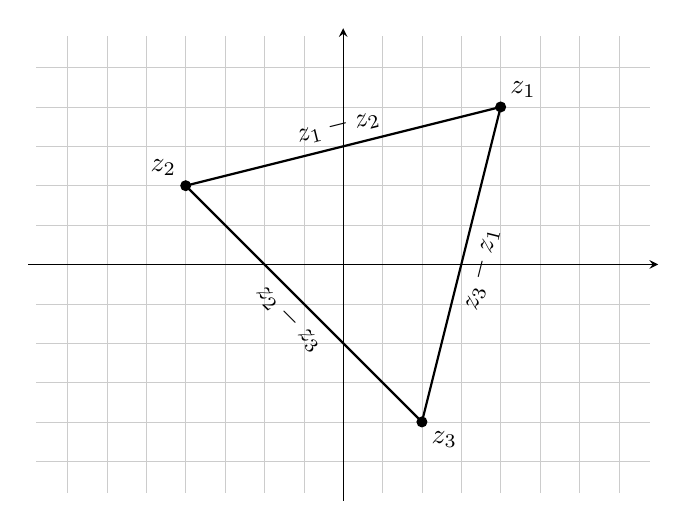
\begin{tikzpicture}
      \def\a{2};
      \def\b{2};
      \def\c{-2};
      \def\d{1};
      \def\e{1};
      \def\f{-2};
      \draw [black!20,step=0.5,very thin] (-4+0.1,-3+0.1) grid (4-0.1,3-0.1);
      \draw[-stealth] (-4,0) -- (4,0);
      \draw[-stealth] (0,-3) -- (0,3);
      \fill (\a,\b) circle (2pt);
      \draw (\a,\b) node [above right] {$z_1$};
      \fill (\c,\d) circle (2pt);
      \draw (\c,\d) node [above left] {$z_2$};
      \fill (\e,\f) circle (2pt);
      \draw (\e,\f) node [below right] {$z_3$};
      \draw[thick] (\a,\b) -- (\c,\d) node [sloped,midway,above] {$\abs{z_1-z_2}$};
      \draw[thick] (\c,\d) -- (\e,\f) node [sloped,midway,below] {$\abs{z_2-z_3}$};
      \draw[thick] (\e,\f) -- (\a,\b) node [sloped,midway,below] {$\abs{z_3-z_1}$};
    \end{tikzpicture}
  \end{center}
\end{lemma}

\subsection{Forma trigonometrica}

Sia $\complex\ni z\neq0$. Allora:
$$z=z\frac{\abs{z}}{\abs{z}}=\abs{z}\frac{z}{\abs{z}}=\r w$$
$$\r=\abs{z}\quad w=\frac{z}{\abs{z}}$$
$$\abs{w}=\abs{\frac{z}{\abs{z}}}=\frac{\abs{z}}{\abs{\abs{z}}}=\frac{\abs{z}}{\abs{z}}=1$$
$$w=\(\cos\t,\sin\t\)$$
$$z=\r\(\cos\t+i\sin\t\)$$
$$\re\(z\)=\r\cos\t$$
$$\im\(z\)=\r\sin\t$$
$$\t\walrus \arg\(z\)$$

\begin{center}
  \begin{tikzpicture}
    \def\a{2.5};
    \def\b{2};
    \draw [black!20,step=0.5,very thin] (-4+0.1,-3+0.1) grid (4-0.1,3-0.1);
    \node (z) at (\a,\b) [above right] {$z$};
    \node (X) at (1,0) {};
    \node (Y) at (0,1) {};
    \node (O) at (0,0) {};
    \draw[-stealth] (-4,0) -- (4,0) node [right] {$\re$};
    \draw[-stealth] (0,-3) -- (0,3) node [above] {$\im$};
    \fill (0,0) circle (2pt);
    \fill (\a,\b) circle (2pt);
    \draw[dashed] (0,\b) -- (\a,\b);
    \draw[dashed] (\a,0) -- (\a,\b);
    \draw (\a,0) node [below] {$a$};
    \draw (0,\b) node [left] {$b$};
    \draw[thin] (0,0) circle (1);
    \draw[thick] (0,0) -- (\a,\b) node [sloped,midway,above] {$\r$};
    \draw[densely dotted] (0,0) ++(20:{sqrt(\a*\a+\b*\b)}) arc (20:60:{sqrt(\a*\a+\b*\b)});
    \pic [draw,-stealth,"$\t$",angle eccentricity=1.5] {angle = X--O--z};
  \end{tikzpicture}
\end{center}

\begin{theorem}[I formula di De Moivre]
  $$z_1=\r_1\(\cos\t_1+i\sin\t_1\)$$
  $$z_2=\r_2\(\cos\t_2+i\sin\t_2\)$$
  $$z_1z_2=\r_1\r_2\(\cos\(\t_1+\t_2\)+i\sin\(\t_1+\t_2\)\)$$
  \begin{center}
    \begin{tikzpicture}
      \def\a{1.5};
      \def\b{1};
      \def\c{-2};
      \def\d{0.25};
      \draw [black!20,step=0.5,very thin] (-4+0.1,-3+0.1) grid (4-0.1,3-0.1);
      \coordinate (X) at (1,0);
      \coordinate (Y) at (0,1);
      \coordinate (O) at (0,0);
      \coordinate (z) at (\a,\b);
      \coordinate (w) at (\c,\d);
      \coordinate (zw) at (\a*\c-\b*\d,\a*\d+\b*\c);
      \draw[-stealth] (-4,0) -- (4,0);
      \draw[-stealth] (0,-3) -- (0,3);
      \node at (z) [above right] {$z_1$};
      \node at (w) [above left] {$z_2$};
      \node at (zw) [below left] {$z_1z_2$};
      \draw[thick] (O) -- (z) node [sloped,midway,above] {$\r_1$};
      \draw[thick] (O) -- (w) node [sloped,midway,above] {$\r_2$};
      \draw[thick] (O) -- (zw) node [sloped,midway,above] {$\r_1\r_2$};
      \fill (O) circle (2pt);
      \fill (z) circle (2pt);
      \fill (w) circle (2pt);
      \fill (zw) circle (2pt);
      \pic [draw,-stealth,"$\t_1$",angle eccentricity=1.3,angle radius=9mm] {angle = X--O--z};
      \pic [draw,-stealth,"$\t_2$",angle eccentricity=1.5,angle radius=6mm] {angle = X--O--w};
      \pic [draw,-stealth,angle radius=3mm] {angle = X--O--zw};
    \end{tikzpicture}
  \end{center}
\end{theorem}
\begin{proof}
  \begin{align*}
    z_1z_2 & =\r_1\(\cos\t_1+i\sin\t_1\)\r_2\(\cos\t_2+i\sin\t_2\)                              \\
           & =\r_1\r_2\(\cos\t_1\cos\t_2+i\cos\t_1\sin\t_2+i\sin\t_1\cos\t_2-\sin\t_1\sin\t_2\) \\
           & =\r_1\r_2\(\cos\(\t_1+\t_2\)+i\sin\(\t_1+\t_2\)\)                                  
  \end{align*}
\end{proof}

\begin{corollary}
  $$z=\r\(\cos\t+i\sin\t\)$$
  $$z^n=\r^n\(\cos n\t+i\sin n\t\)$$
\end{corollary}

\begin{theorem}[II formula di De Moivre]
  Sia $\complex\setminus\left\{ 0 \right\}\ni w\walrus\r\(\cos\t+i\sin\t\)$ e $n\in\mathbb{N}\setminus\left\{ 0 \right\}$. Allora l'equazione $z^n=w$ ha esattamente $n$ soluzioni, ossia:
  $$z_k^n=w\quad \forall k\in\rintv{0}{n}$$
  In particolare:
  $$z_k=\r^{\nicefrac{1}{n}}\(\cos\t_k+i\sin\t_k\)\quad \t_k=\frac{\t}{n}+\frac{2\pi}{n}k$$
  \begin{center}
    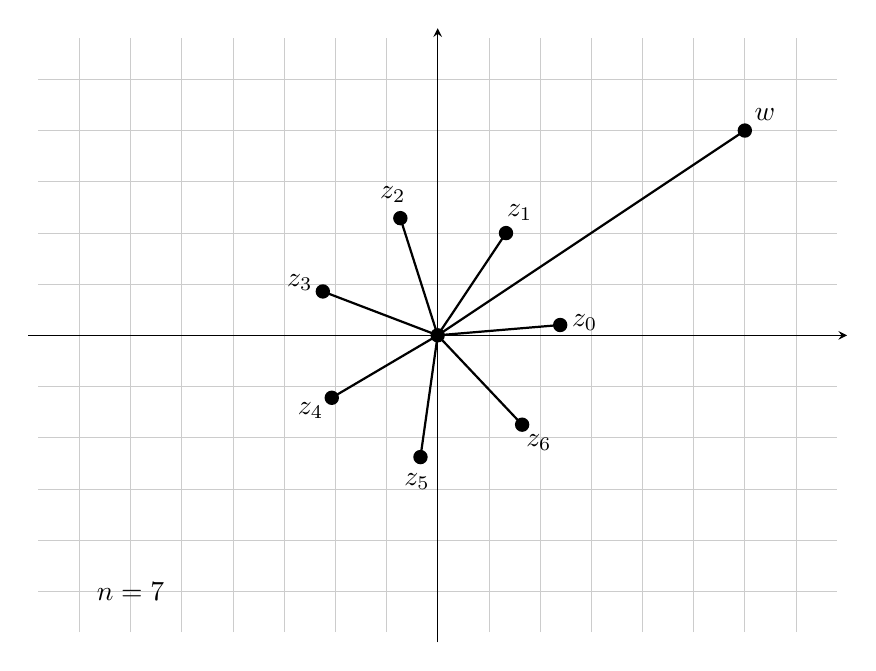
\begin{tikzpicture}[scale=1.3]
      \def\a{3};
      \def\b{2};
      \def\n{7};
      \draw [black!20,step=0.5,very thin] (-4+0.1,-3+0.1) grid (4-0.1,3-0.1);
      \draw[-stealth] (-4,0) -- (4,0);
      \draw[-stealth] (0,-3) -- (0,3);
      \coordinate (X) at (1,0);
      \coordinate (Y) at (0,1);
      \coordinate (O) at (0,0);
      \coordinate (w) at (\a,\b);
      \fill (O) circle (2pt);
      \fill (w) circle (2pt);
      \node at (w) [above right] {$w$};
      \draw[thick] (O) -- (w);
      \pgfmathsetmacro{\r}{sqrt(\a*\a+\b*\b)};
      \pgfmathsetmacro{\t}{atan(\b/\a)};
      \pgfmathsetmacro{\rk}{\r^(1/\n)};
      \foreach \k [parse=true] in {0,...,\n-1} {
          \pgfmathsetmacro{\tk}{\t/\n+360*\k/\n};
          \pgfmathsetmacro{\x}{\rk*cos(\tk)};
          \pgfmathsetmacro{\y}{\rk*sin(\tk)};
          \coordinate (z) at (\x,\y);
          \fill (z) circle (2pt);
          \draw[thick] (O) -- (z) node [pos=1.2] {$z_{\k}$};
        }
      \node at (-3,-2.5) {$n={\n}$};
    \end{tikzpicture}
  \end{center}
\end{theorem}
\begin{proof}
  \begin{align*}
    z_k^n & =\(\r^{\nicefrac{1}{n}}\(\cos\t_k+i\sin\t_k\)\)^n \\
          & =\r^{\nicefrac{n}{n}}\(\cos n\t_k+i\sin n\t_k\)   \\
          & =\r\(\cos\(\t+2k\pi\)+i\sin\(\t+2k\pi\)\)         \\
          & =\r\(\cos\t+i\sin\t\)                             \\
          & =w                                                
  \end{align*}
\end{proof}

\begin{observation}
  Le $n$ radici $n$--esime di $w\in\complex\setminus\left\{ 0 \right\}$ sono i vertici di un poligono regolare di $n$ lati, inscritto nella circonferenza centrata in $0\in\complex$ e di raggio $\r^{\nicefrac{1}{n}}$.
  \begin{center}
    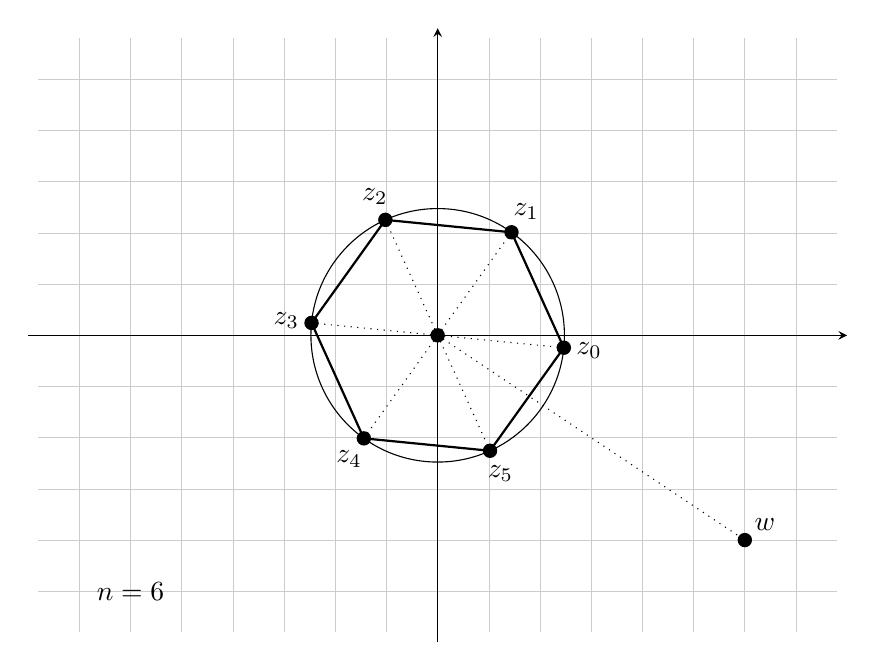
\begin{tikzpicture}[scale=1.3]
      \def\a{3};
      \def\b{-2};
      \def\n{6};
      \draw [black!20,step=0.5,very thin] (-4+0.1,-3+0.1) grid (4-0.1,3-0.1);
      \draw[-stealth] (-4,0) -- (4,0);
      \draw[-stealth] (0,-3) -- (0,3);
      \coordinate (X) at (1,0);
      \coordinate (Y) at (0,1);
      \coordinate (O) at (0,0);
      \coordinate (w) at (\a,\b);
      \fill (O) circle (2pt);
      \fill (w) circle (2pt);
      \node at (w) [above right] {$w$};
      \draw[dotted] (O) -- (w);
      \pgfmathsetmacro{\r}{sqrt(\a*\a+\b*\b)};
      \pgfmathsetmacro{\t}{atan(\b/\a)};
      \pgfmathsetmacro{\rk}{\r^(1/\n)};
      \foreach \k [parse=true,remember=\k as \lk (initially (\n-1))] in {0,...,\n-1} {
          \pgfmathsetmacro{\tk}{\t/\n+360*\k/\n};
          \pgfmathsetmacro{\x}{\rk*cos(\tk)};
          \pgfmathsetmacro{\y}{\rk*sin(\tk)};
          \pgfmathsetmacro{\ltk}{\t/\n+360*\lk/\n};
          \pgfmathsetmacro{\lx}{\rk*cos(\ltk)};
          \pgfmathsetmacro{\ly}{\rk*sin(\ltk)};
          \coordinate (z) at (\x,\y);
          \fill (z) circle (2pt);
          \draw[dotted] (O) -- (z) node [pos=1.2] {$z_{\k}$};
          \draw[thick] (z) -- (\lx,\ly);
        }
      \node at (-3,-2.5) {$n={\n}$};
      \draw (O) circle (\rk);
    \end{tikzpicture}
  \end{center}
\end{observation}

\begin{definition}[Polinomio]
  Un \textbf{polinomio} è una funzione:
  $$P_n:\complex\to\complex\quad P_n\(z\)\walrus\sum_{i=0}^nc_iz^i$$
  $n$ è detto \textbf{grado} del polinomio e $\left\{ c_i:0\le i\le n \right\}\subset\complex$ è l'insieme dei \textbf{coefficienti} del polinomio.
\end{definition}

\begin{definition}[Equazione algebrica]
  Sia $P_n$ un polinomio di grado $n$. L'equazione $P(z)=0$ prende il nome di \textbf{equazione algebrica}. 
\end{definition}

\begin{theorem}[Teorema fondamentale dell'algebra]
  Un'equazione algebrica di grado $n$ ha $N$ soluzioni $w\walrus\left\{ w_i:1\le i\le N \right\}$, cui corrispondono gli indici $m\walrus\left\{ m_i:1\le i\le N \right\}$ tali per cui $\sum m_i=n$. Tali indici si dicono \textbf{molteplicità} di $w$.
  $$P_n(z)=c_n\(z-w_1\)^{m_1}\cdots\(z-w_N\)^{m_N}$$
\end{theorem}

\subsection{Trasformazioni del piano di Gauss}

\subsubsection*{Traslazione}

Sia $z_0\in\complex$.
$$T:\complex\to\complex\quad T\(z\)\walrus z+z_0$$
\begin{center}
  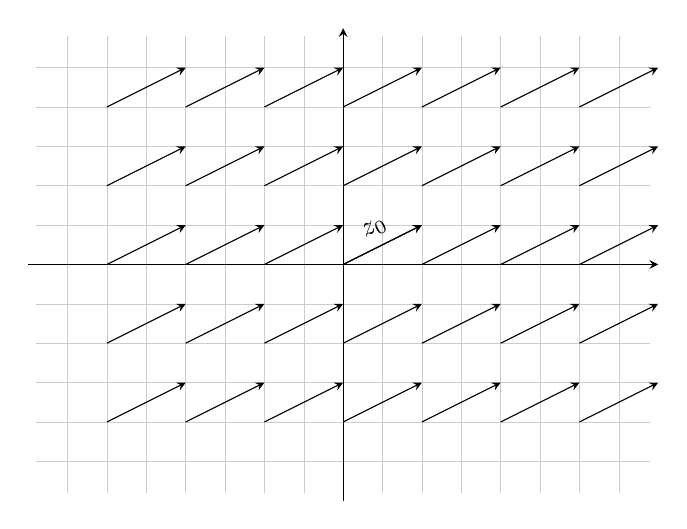
\begin{tikzpicture}
    \def\a{1};
    \def\b{0.5};
    \draw [black!20,step=0.5,very thin] (-4+0.1,-3+0.1) grid (4-0.1,3-0.1);
    \draw[-stealth] (-4,0) -- (4,0);
    \draw[-stealth] (0,-3) -- (0,3);
    \coordinate (X) at (1,0);
    \coordinate (Y) at (0,1);
    \coordinate (O) at (0,0);
    \coordinate (z0) at (\a,\b);
    \draw[-stealth] (O) -- (z0) node [sloped,midway,above] {$z_0$};
    \foreach \x in {-3,...,3}
    \foreach \y in {-2,...,2} {
        \coordinate (z) at (\x,\y); 
        % \fill (z) circle (1pt);
        % \fill (z) +(z0) circle (1pt);
        \draw[-stealth] (z) -- +(z0);
      }
  \end{tikzpicture}
\end{center}

\subsubsection*{Rotazione}

Sia $w\in\complex:\abs{w}=1$.
$$R:\complex\to\complex\quad R\(z\)\walrus wz$$
\begin{center}
  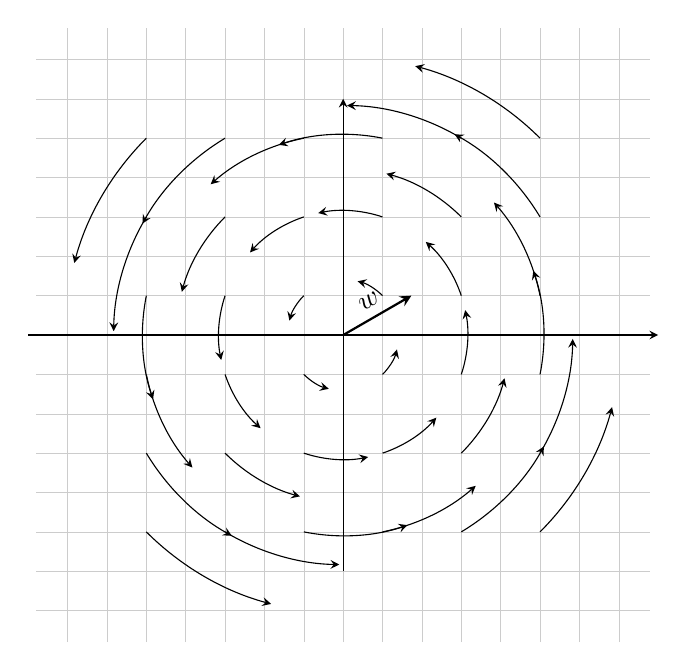
\begin{tikzpicture}
    \pgfmathsetmacro{\t}{30};
    \pgfmathsetmacro{\a}{cos(\t)};
    \pgfmathsetmacro{\b}{sin(\t)};
    \draw [black!20,step=0.5,very thin] (-4+0.1,-4+0.1) grid (4-0.1,4-0.1);
    \draw[-stealth] (-4,0) -- (4,0);
    \draw[-stealth] (0,-3) -- (0,3);
    \coordinate (X) at (1,0);
    \coordinate (Y) at (0,1);
    \coordinate (O) at (0,0);
    \coordinate (w) at (\a,\b);
    \draw[thick,-stealth] (O) -- (w) node [sloped,midway,above] {$w$};
    \foreach \x in {-2.5,...,2.5}
    \foreach \y in {-2.5,...,2.5} {
        \coordinate (z) at (\x,\y); 
        \coordinate (r) at (\a*\x-\b*\y,\a*\y+\b*\x);
        \pgfmathsetmacro{\d}{sqrt(\x*\x+\y*\y)};
        \pgfmathsetmacro{\c}{atan2(\y,\x)};
        \pgfmathsetmacro{\s}{\c+\t};
        % \fill (z) circle (1pt);
        % \fill (r) circle (1pt);
        \pgfmathparse{\x==0&&\y==0};
        \ifnum\pgfmathresult=0
          \draw[-stealth] (O) +(\c:\d) arc (\c:\s:\d);
        \fi
      }
  \end{tikzpicture}
\end{center}

\subsubsection*{Dilatazione}

Sia $\reals\ni\r>0$.
$$D:\complex\to\complex\quad D\(z\)\walrus \r z$$
\begin{center}
  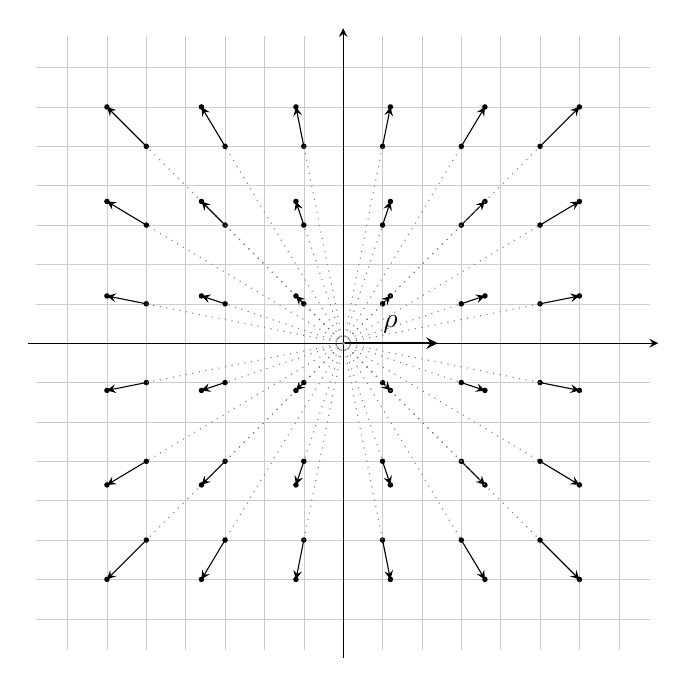
\begin{tikzpicture}
    \def\r{1.2};
    \draw [black!20,step=0.5,very thin] (-4+0.1,-4+0.1) grid (4-0.1,4-0.1);
    \draw[-stealth] (-4,0) -- (4,0);
    \draw[-stealth] (0,-4) -- (0,4);
    \coordinate (X) at (1,0);
    \coordinate (Y) at (0,1);
    \coordinate (O) at (0,0);
    \coordinate (w) at (\r,0);
    \draw[thick,-stealth] (O) -- (w) node [sloped,midway,above] {$\rho$};
    \foreach \x in {-2.5,...,2.5}
    \foreach \y in {-2.5,...,2.5} {
        \coordinate (z) at (\x,\y); 
        \coordinate (d) at (\x*\r,\y*\r);
        \fill (z) circle (1pt);
        \fill (d) circle (1pt);
        \draw[gray,dotted] (O) -- (z);
        \draw[-stealth] (z) -- (d);
      }
  \end{tikzpicture}
\end{center}

\subsubsection*{Inversione}

$$I:\complex\to\complex\quad I\(z\)\walrus -z$$
\begin{center}
  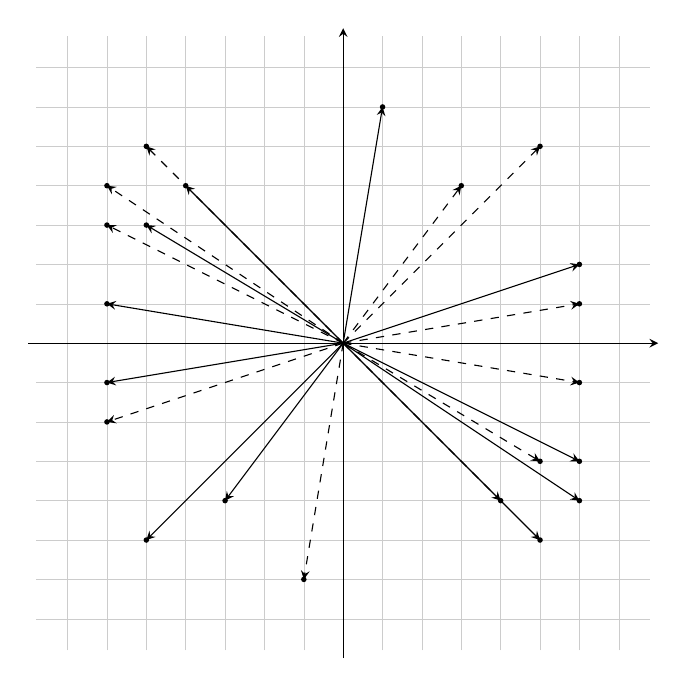
\begin{tikzpicture}
    \draw [black!20,step=0.5,very thin] (-4+0.1,-4+0.1) grid (4-0.1,4-0.1);
    \draw[-stealth] (-4,0) -- (4,0);
    \draw[-stealth] (0,-4) -- (0,4);
    \coordinate (X) at (1,0);
    \coordinate (Y) at (0,1);
    \coordinate (O) at (0,0);
    \foreach \i in {0,...,10} {
        \pgfmathrandominteger{\x0}{0}{12};
        \pgfmathrandominteger{\y0}{0}{12};
        \pgfmathsetmacro{\x}{\x0/2-3};
        \pgfmathsetmacro{\y}{\y0/2-3};
        \coordinate (z) at (\x,\y); 
        \coordinate (w) at (-\x,-\y);
        \fill (z) circle (1pt);
        \fill (w) circle (1pt);
        \draw [-stealth,dashed] (O) -- (z);
        \draw [-stealth] (O) -- (w);
      }
  \end{tikzpicture}
\end{center}

\subsubsection*{Simmetria con l'asse reale}

$$S:\complex\to\complex\quad S\(z\)\walrus \bar{z}$$
\begin{center}
  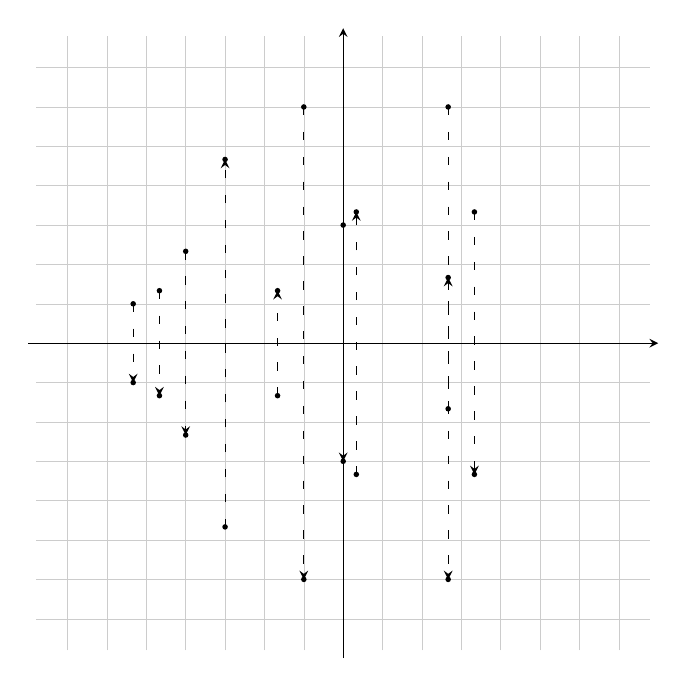
\begin{tikzpicture}
    \draw [black!20,step=0.5,very thin] (-4+0.1,-4+0.1) grid (4-0.1,4-0.1);
    \draw[-stealth] (-4,0) -- (4,0);
    \draw[-stealth] (0,-4) -- (0,4);
    \coordinate (X) at (1,0);
    \coordinate (Y) at (0,1);
    \coordinate (O) at (0,0);
    \foreach \i in {0,...,10} {
        \pgfmathrandominteger{\x0}{0}{6*6};
        \pgfmathrandominteger{\y0}{0}{6*6};
        \pgfmathsetmacro{\x}{\x0/6-3};
        \pgfmathsetmacro{\y}{\y0/6-3};
        \coordinate (z) at (\x,\y); 
        \coordinate (w) at (\x,-\y);
        \fill (z) circle (1pt);
        \fill (w) circle (1pt);
        \draw [-stealth,loosely dashed] (z) -- (w);
      }
  \end{tikzpicture}
\end{center}

\subsubsection*{Funzione di Joukowsky}

$$f:\complex\setminus\left\{ 0 \right\}\to\complex\quad f\(z\)\walrus z+\frac{1}{z}$$

\begin{example}
  $$\complex\ni z:\abs{z}=1$$
  $$f\(z\)=z+\frac{1}{z}=z+\frac{\bar{z}}{\abs{z}^2}=z+\bar{z}=2\re\(z\)$$
\end{example}

% TODO
% il disegno è più complicato: si deve disegnare la trasformazione come due grafici, il primo mostra una circonferenza e delle rette, parallele all'asse delle ascisse, che vengono curvate dalla circonferenza (similmente a quanto accade con la gravità), il secondo mostra gli effetti della trasformazione, ossia un segmento dove prima c'era la circonferenza e rette parallele all'asse reale dove prima c'erano curve. il tutto è completato da frecce circolari che indicano il passaggio diretto e inverso della trasformazione (quindi, da sinistra a destra una freccia f, da destra a sinistra una freccia f^{-1})

\begin{observation}
  La funzione non è un'isometria, perciò non conserva le distanze, ma bensì gli angoli.
\end{observation}

\subsection{Forma esponenziale}

$$z=\r\(\cos\t+i\sin\t\)=\r e^{i\t}$$
$$zw=\r_1\r_2\(\cos\(\t_1+\t_2\)+i\sin\(\t_1+\t_2\)\)=\r_1\r_2 e^{i\(\t_1+\t_2\)}$$